\documentclass{standalone}
\usepackage{tikz}
\usepackage{xcolor}
\usetikzlibrary{patterns, positioning}
\usetikzlibrary{shapes.misc}
\usepackage[outline]{contour}
\contourlength{1.5pt} 


\begin{document}
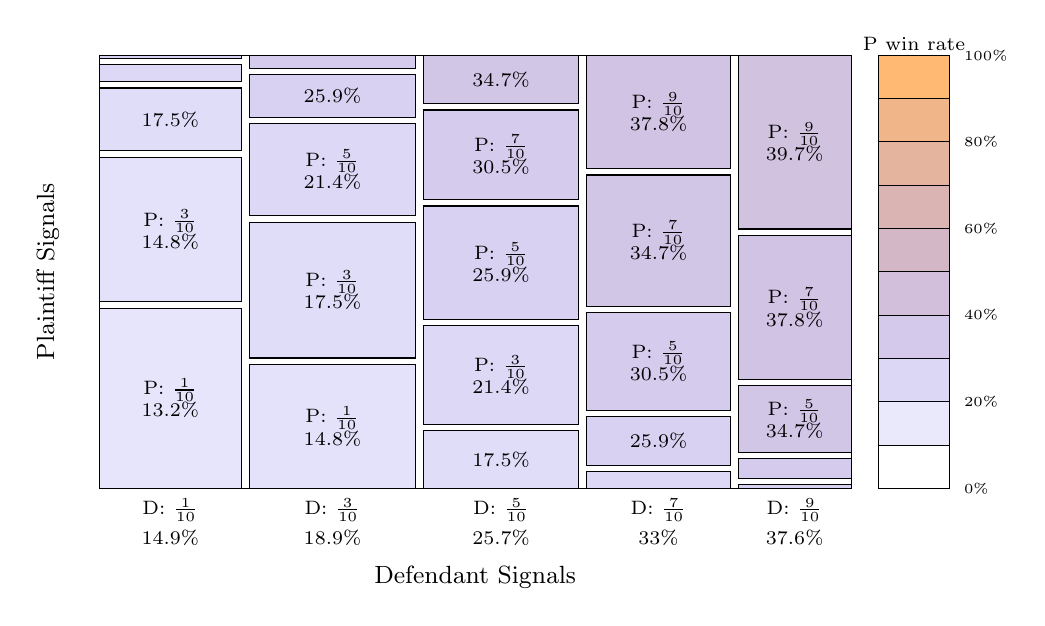
\begin{tikzpicture}
\newcommand{\DFractionOffset}{0.4}
\newcommand{\AxisLabelYAdjust}{-0.235}
\draw[draw=black] (0.6,2) rectangle (10.15,7.5);
\draw[fill=blue!87!orange!13!white!84!white, draw=black] (0.6,2) rectangle (2.4096,4.289);
\draw (1.5047798846091756, 3.1445112837205462) node[font=\scriptsize, text=black, align=center] {P: $\frac{1}{10}$\\ 13.2\%};
\draw[fill=blue!85!orange!15!white!83!white, draw=black] (0.6,4.369) rectangle (2.4096,6.2056);
\draw (1.5047798846091756, 5.2873019683578555) node[font=\scriptsize, text=black, align=center] {P: $\frac{3}{10}$\\ 14.8\%};
\draw[fill=blue!82!orange!18!white!82!white, draw=black] (0.6,6.2856) rectangle (2.4096,7.0852);
\draw (1.5047798846091756, 6.68538634594268) node[font=\scriptsize, text=black, align=center] {17.5\%};
\draw[fill=blue!79!orange!21!white!81!white, draw=black] (0.6,7.1652) rectangle (2.4096,7.3809);
\draw[fill=blue!74!orange!26!white!79!white, draw=black] (0.6,7.4609) rectangle (2.4096,7.5);
\draw (1.5047798846091756, 1.6) node[anchor=north, font=\scriptsize, text=black] {14.9\%};
\draw (1.5047798846091756, {1.6 + \DFractionOffset}) node[anchor=north, font=\scriptsize, text=black] {D: $\frac{1}{10}$};
\draw[fill=blue!85!orange!15!white!83!white, draw=black] (2.5096,2) rectangle (4.6179,3.5763);
\draw (3.5637184973432694, 2.7881552447782765) node[font=\scriptsize, text=black, align=center] {P: $\frac{1}{10}$\\ 14.8\%};
\draw[fill=blue!82!orange!18!white!82!white, draw=black] (2.5096,3.6563) rectangle (4.6179,5.3819);
\draw (3.5637184973432694, 4.519095344676105) node[font=\scriptsize, text=black, align=center] {P: $\frac{3}{10}$\\ 17.5\%};
\draw[fill=blue!79!orange!21!white!81!white, draw=black] (2.5096,5.4619) rectangle (4.6179,6.635);
\draw (3.5637184973432694, 6.048428403368227) node[font=\scriptsize, text=black, align=center] {P: $\frac{5}{10}$\\ 21.4\%};
\draw[fill=blue!74!orange!26!white!79!white, draw=black] (2.5096,6.715) rectangle (4.6179,7.2515);
\draw (3.5637184973432694, 6.983227815745896) node[font=\scriptsize, text=black, align=center] {25.9\%};
\draw[fill=blue!70!orange!30!white!78!white, draw=black] (2.5096,7.3315) rectangle (4.6179,7.5);
\draw (3.5637184973432694, 1.6) node[anchor=north, font=\scriptsize, text=black] {18.9\%};
\draw (3.5637184973432694, {1.6 + \DFractionOffset}) node[anchor=north, font=\scriptsize, text=black] {D: $\frac{3}{10}$};
\draw[fill=blue!82!orange!18!white!82!white, draw=black] (4.7179,2) rectangle (6.6924,2.7328);
\draw (5.70515831192796, 2.3663956553173993) node[font=\scriptsize, text=black, align=center] {17.5\%};
\draw[fill=blue!79!orange!21!white!81!white, draw=black] (4.7179,2.8128) rectangle (6.6924,4.0654);
\draw (5.70515831192796, 3.4390718266317104) node[font=\scriptsize, text=black, align=center] {P: $\frac{3}{10}$\\ 21.4\%};
\draw[fill=blue!74!orange!26!white!79!white, draw=black] (4.7179,4.1454) rectangle (6.6924,5.586);
\draw (5.70515831192796, 4.865685933057508) node[font=\scriptsize, text=black, align=center] {P: $\frac{5}{10}$\\ 25.9\%};
\draw[fill=blue!70!orange!30!white!78!white, draw=black] (4.7179,5.666) rectangle (6.6924,6.8059);
\draw (5.70515831192796, 6.2359395771386) node[font=\scriptsize, text=black, align=center] {P: $\frac{7}{10}$\\ 30.5\%};
\draw[fill=blue!65!orange!35!white!77!white, draw=black] (4.7179,6.8859) rectangle (6.6924,7.5);
\draw (5.70515831192796, 7.192929815395404) node[font=\scriptsize, text=black, align=center] {34.7\%};
\draw (5.70515831192796, 1.6) node[anchor=north, font=\scriptsize, text=black] {25.7\%};
\draw (5.70515831192796, {1.6 + \DFractionOffset}) node[anchor=north, font=\scriptsize, text=black] {D: $\frac{5}{10}$};
\draw[fill=blue!79!orange!21!white!81!white, draw=black] (6.7924,2) rectangle (8.6163,2.2141);
\draw[fill=blue!74!orange!26!white!79!white, draw=black] (6.7924,2.2941) rectangle (8.6163,2.9142);
\draw (7.704359535730165, 2.6041565175958796) node[font=\scriptsize, text=black, align=center] {25.9\%};
\draw[fill=blue!70!orange!30!white!78!white, draw=black] (6.7924,2.9942) rectangle (8.6163,4.2283);
\draw (7.704359535730165, 3.611266917110441) node[font=\scriptsize, text=black, align=center] {P: $\frac{5}{10}$\\ 30.5\%};
\draw[fill=blue!65!orange!35!white!77!white, draw=black] (6.7924,4.3083) rectangle (8.6163,5.9801);
\draw (7.704359535730165, 5.144170949817444) node[font=\scriptsize, text=black, align=center] {P: $\frac{7}{10}$\\ 34.7\%};
\draw[fill=blue!62!orange!38!white!76!white, draw=black] (6.7924,6.0601) rectangle (8.6163,7.5);
\draw (7.704359535730165, 6.780028408764753) node[font=\scriptsize, text=black, align=center] {P: $\frac{9}{10}$\\ 37.8\%};
\draw (7.704359535730165, 1.6) node[anchor=north, font=\scriptsize, text=black] {33\%};
\draw (7.704359535730165, {1.6 + \DFractionOffset}) node[anchor=north, font=\scriptsize, text=black] {D: $\frac{7}{10}$};
\draw[fill=blue!74!orange!26!white!79!white, draw=black] (8.7163,2) rectangle (10.15,2.0493);
\draw[fill=blue!70!orange!30!white!78!white, draw=black] (8.7163,2.1293) rectangle (10.15,2.3771);
\draw[fill=blue!65!orange!35!white!77!white, draw=black] (8.7163,2.4571) rectangle (10.15,3.3029);
\draw (9.433139836536299, 2.8800130572555047) node[font=\scriptsize, text=black, align=center] {P: $\frac{5}{10}$\\ 34.7\%};
\draw[fill=blue!62!orange!38!white!76!white, draw=black] (8.7163,3.3829) rectangle (10.15,5.2147);
\draw (9.433139836536299, 4.298797421001675) node[font=\scriptsize, text=black, align=center] {P: $\frac{7}{10}$\\ 37.8\%};
\draw[fill=blue!60!orange!40!white!75!white, draw=black] (8.7163,5.2947) rectangle (10.15,7.5);
\draw (9.433139836536299, 6.397337807848339) node[font=\scriptsize, text=black, align=center] {P: $\frac{9}{10}$\\ 39.7\%};
\draw (9.433139836536299, 1.6) node[anchor=north, font=\scriptsize, text=black] {37.6\%};
\draw (9.433139836536299, {1.6 + \DFractionOffset}) node[anchor=north, font=\scriptsize, text=black] {D: $\frac{9}{10}$};
\node[font=\small, text=black] at (5.375, {1.1 + \AxisLabelYAdjust}) {Defendant Signals};
\node[font=\small, text=black, rotate=90] at (-0.050000000000000044, 4.75) {Plaintiff Signals};
\draw[draw=black] (10.5,2) rectangle (11.4,7.5);
\draw (10.95, 7.65) node[font=\scriptsize, text=black] {P win rate};
\draw[fill=blue!100!orange!0!white!88!white, draw=black] (10.5,2) rectangle (11.4,2.55);
\draw[fill=blue!89!orange!11!white!84!white, draw=black] (10.5,2.55) rectangle (11.4,3.1);
\draw[fill=blue!78!orange!22!white!81!white, draw=black] (10.5,3.1) rectangle (11.4,3.65);
\draw[fill=blue!67!orange!33!white!77!white, draw=black] (10.5,3.65) rectangle (11.4,4.2);
\draw[fill=blue!56!orange!44!white!73!white, draw=black] (10.5,4.2) rectangle (11.4,4.75);
\draw[fill=blue!44!orange!56!white!70!white, draw=black] (10.5,4.75) rectangle (11.4,5.3);
\draw[fill=blue!33!orange!67!white!66!white, draw=black] (10.5,5.3) rectangle (11.4,5.85);
\draw[fill=blue!22!orange!78!white!62!white, draw=black] (10.5,5.85) rectangle (11.4,6.4);
\draw[fill=blue!11!orange!89!white!59!white, draw=black] (10.5,6.4) rectangle (11.4,6.95);
\draw[fill=blue!0!orange!100!white!55!white, draw=black] (10.5,6.95) rectangle (11.4,7.5);
\draw (11.46, 2) node[anchor=west, font=\tiny, text=black] {0\%};
\draw (11.46, 3.1) node[anchor=west, font=\tiny, text=black] {20\%};
\draw (11.46, 4.2) node[anchor=west, font=\tiny, text=black] {40\%};
\draw (11.46, 5.3) node[anchor=west, font=\tiny, text=black] {60\%};
\draw (11.46, 6.4) node[anchor=west, font=\tiny, text=black] {80\%};
\draw (11.46, 7.5) node[anchor=west, font=\tiny, text=black] {100\%};


\end{tikzpicture}
\end{document}